% cd /storage/emulated/0/Documents/documents/latex/1920/Grade-8/1st/rectangular-coordinate-system && pdflatex ps-rectangular-coordinate-system.tex && termux-open ps-rectangular-coordinate-system.pdf

% cd /storage/emulated/0/Documents/documents/latex/1920/Grade-8/1st/rectangular-coordinate-system && clean-tex ps-rectangular-coordinate-system-input1.tex


% cd /storage/emulated/0/Documents/documents/latex/1920/Grade-8/1st/rectangular-coordinate-system && convert -density 600 ps-rectangular-coordinate-system.pdf -crop 2200x1700 -quality 100 -verbose ps-rectangular-coordinate-system%02d.png

%2480.5x3508 portrait 2x2 2550x3300
%3508x2480.5 landscape 2x2 3300x2550 
%1653.7x2338.7 portrait 3x3 1700x2200
%landscape 3x3 2200x1700

% cd /storage/emulated/0/Documents/documents/latex/1819/grade10/visual/4th/rectangular-coordinate-system && while inotifywait -e close_write ps-rectangular-coordinate-system*.tex; do touch /storage/emulated/0/Android/data/com.termux/files/launch-termux.txt && printf '1' > /storage/emulated/0/Android/data/com.termux/files/launch-termux.txt && pdflatex ps-rectangular-coordinate-system.tex && termux-open ps-rectangular-coordinate-system.pdf; done

% cd /host-rootfs/storage/emulated/0/Documents/documents/latex/1819/grade10/visual/4th/rectangular-coordinate-system && while inotifywait -e close_write ps-rectangular-coordinate-system*.tex; do pdflatex ps-rectangular-coordinate-system.tex  && printf "/storage/emulated/0/Documents/documents/latex/1819/grade10/visual/4th/rectangular-coordinate-system/ps-rectangular-coordinate-system.pdf" > /host-rootfs/storage/emulated/0/GNURoot/home/Scripts/file-to-launch.txt; done


\documentclass[10pt]{article}
\usepackage[letterpaper, landscape, right=0.25in, left=0.4in, top=0.25in, bottom=0.25in]{geometry}
\usepackage{xcolor}
\usepackage{anyfontsize}
\usepackage{enumitem}
\usepackage{multicol}
\usepackage{amsmath}
%\usepackage{amsfonts,dsfont}% for \mathds 
\usepackage{tabularx} 
\usepackage{gensymb}
\usepackage{multirow}
\usepackage{graphicx, tipa}
\usepackage{tikz}
\usetikzlibrary{angles,quotes}
\usepackage{pgfplots} 
\usetikzlibrary{calc}
\pgfplotsset{compat=newest}
\usetikzlibrary{arrows.meta}
\usetikzlibrary{intersections}
\usetikzlibrary{decorations.pathreplacing}
\usepackage{flafter}
\usepackage{amsmath,amssymb,cancel,units}
\usepackage{microtype} % nicer output 
\usepackage{hfoldsty} % nicer output 
\usepackage{fixltx2e} 
\usepackage{mathptmx}
%\usepackage{booktabs}
\usepackage{numprint}
\usepackage[utf8]{inputenc} 
\usepackage[T1]{fontenc}
%\usepackage{siunitx} 
%\sisetup{detect-all}


\def\radA{3.6cm}

\def\radB{3.6cm}

%\def\thirdrad{8cm}

\pagenumbering{gobble}
%\linespread{0.9}
\newcommand{\vspce}{\vspace{0.75ex}}
\newcommand{\hspce}{\hspace{0.5em}}
\newcommand{\blank}{\underline{\hspace{2em}}}%{\rule{1em}{0.15ex}}
\newcommand{\arc}[1]{{% 
\setbox9=\hbox{#1}% 
\ooalign{\resizebox{\wd9}{\height}{\texttoptiebar{\phantom{A}}}\cr#1}}}

\newcolumntype{C}{ >{\centering\arraybackslash} X}




\begin{document}
\boldmath
{\fontsize{37}{39}\fontfamily{pnc}\selectfont {

\textbf{Practice Exercises}
%\textbf{Problem Set}

\vspce

%\begin{enumerate}[label = \Alph*. ]
%\item 
A. Name the point that has the coordinates. 

\begin{enumerate}[label = \arabic*. ]
\begin{multicols}{3}

%#1
\item \hspce  (0, 4)
\vspce
%#2
\item \hspce  (-2, -1)
\vspce
%#3
\item \hspce  (0, -6)
\vspce
%#4
\item \hspce  (-5, -4)
\vspce
%#5
\item \hspce  (1, 6)

\end{multicols}
\end{enumerate}


%\end{enumerate} 



%}} 

%\newpage

%{\fontsize{38}{40}\fontfamily{pnc}\selectfont {

B. Write the coordinates of each point. 

\begin{enumerate}[label = \arabic*. ]
\begin{multicols}{3}

\item \hspce E
\item \hspce B
\item \hspce G
\item \hspce D
\item \hspce H
\end{multicols} 
\end{enumerate} 

C. Determine the  quadrant or axis where each point is located. 

\begin{enumerate}[label = \arabic*. ]
\begin{multicols}{3}
\item \hspce A
\item \hspce B
\item \hspce C
\item \hspce D
\item \hspce E
\end{multicols}
\end{enumerate} 

%\newpage 

%\begin{center}

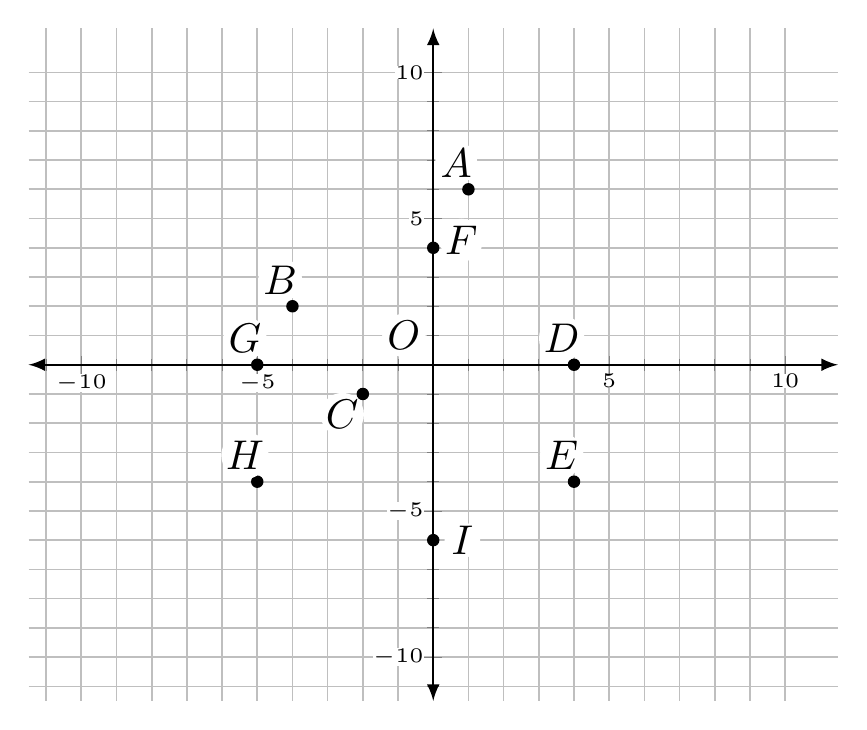
\begin{tikzpicture}[%scale=3.5,
scale=1.5, place/.style={circle, fill=black, inner sep=0pt, outer sep=0pt, minimum size=3pt}, 
point-label/.style={fill=white, circle, inner sep=0pt}
]

\begin{axis}[
    xmin=-11,xmax=11,
    ymin=-11,ymax=11,
    grid=both,
    axis lines=middle,
    minor tick num=4,
    enlargelimits={abs=0.5},
    axis line style={latex-latex},
    ticklabel style={font=\tiny,fill=white, inner sep=0pt},
    xlabel style={at={(ticklabel* cs:1)},anchor=north west},
    ylabel style={at={(ticklabel* cs:1)},anchor=south west}
]

\coordinate (O) at (0,0);
\node[fill=white,circle,inner sep=0pt] (O-label) at ($(O)+(135:10pt)$) {\normalsize $O$};

\node (A) at (1,6) [place] {}; 
\node[point-label] (A-label) at ($(A)+(115:7pt)$) {\normalsize $A$};

\node (B) at (-4,2) [place] {}; 
\node[point-label] (B-label) at ($(B)+(115:7pt)$) {\normalsize $B$};

\node (C) at (-2,-1) [place] {}; 
\node[point-label] (C-label) at ($(C)+(-135:7pt)$) {\normalsize $C$};

\node (D) at (4,0) [place] {}; 
\node[point-label] (D-label) at ($(D)+(115:7pt)$) {\normalsize $D$};

\node (E) at (4,-4) [place] {}; 
\node[point-label] (E-label) at ($(E)+(115:7pt)$) {\normalsize $E$};

\node (F) at (0,4) [place] {}; 
\node[point-label] (F-label) at ($(F)+(15:7pt)$) {\normalsize $F$};

\node (G) at (-5,0) [place] {}; 
\node[point-label] (G-label) at ($(G)+(115:7pt)$) {\normalsize $G$};

\node (H) at (-5,-4) [place] {}; 
\node[point-label] (H-label) at ($(H)+(115:7pt)$) {\normalsize $H$};

\node (I) at (0,-6) [place] {}; 
\node[point-label] (I-label) at ($(I)+(0:7pt)$) {\normalsize $I$};

\end{axis}

 

\end{tikzpicture}
\end{center}  


\newpage

%{\fontsize{38}{40}\fontfamily{pnc}\selectfont {

%\textbf{Practice Exercises}
\textbf{Problem Set}

\vspce

\begin{enumerate}[label = \Alph*. ]
\item Name the point that has the coordinates. 

\begin{enumerate}[label = \arabic*. ]
\begin{multicols}{3}

%#1
\item \hspce  (7, -8)
\vspce
%#2
\item \hspce  (-7, 3)
\vspce
%#3
\item \hspce  (0, 8)
\vspce
%#4
\item \hspce  (-6, -9)
\vspce
%#5
\item \hspce  (2, 9)

\end{multicols}
\end{enumerate}

\item Write the coordinates of each point. 

\begin{enumerate}[label = \arabic*. ]
\begin{multicols}{3}

\item \hspce C
\item \hspce A
\item \hspce F
\item \hspce D
\item \hspce H
\end{multicols} 
\end{enumerate} 

\item Determine the  quadrant or axis where each point is located. 

\begin{enumerate}[label = \arabic*. ]
\begin{multicols}{3}
\item \hspce H
\item \hspce G
\item \hspce F
\item \hspce E
\item \hspce D
\end{multicols}
\end{enumerate} 

\end{enumerate} 

%\newpage 

%\begin{center}

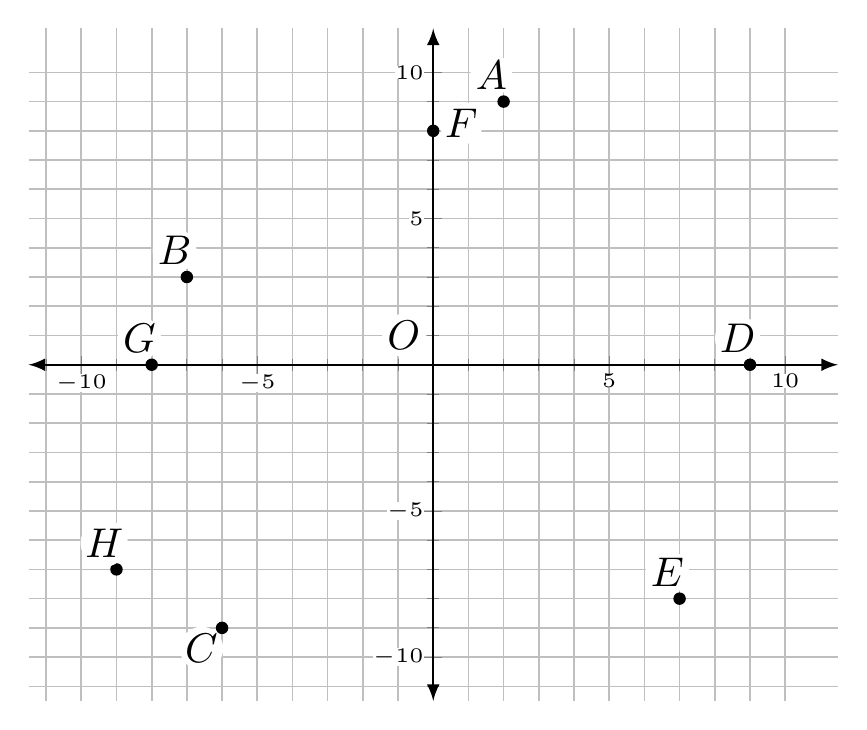
\begin{tikzpicture}[%scale=3.5, 
scale=1.5, place/.style={circle, fill=black, inner sep=0pt, outer sep=0pt, minimum size=3pt}, 
point-label/.style={fill=white, circle,inner sep=0pt}
]

\begin{axis}[
    xmin=-11,xmax=11,
    ymin=-11,ymax=11,
    grid=both,
    axis lines=middle,
    minor tick num=4,
    enlargelimits={abs=0.5},
    axis line style={latex-latex},
    ticklabel style={font=\tiny,fill=white, inner sep=0pt},
    xlabel style={at={(ticklabel* cs:1)},anchor=north west},
    ylabel style={at={(ticklabel* cs:1)},anchor=south west}
]

\coordinate (O) at (0,0);
\node[fill=white,circle,inner sep=0pt] (O-label) at ($(O)+(135:10pt)$) {\normalsize $O$};

\node (A) at (2,9) [place] {}; 
\node[point-label] (A-label) at ($(A)+(115:7pt)$) {\normalsize $A$};

\node (B) at (-7,3) [place] {}; 
\node[point-label] (B-label) at ($(B)+(115:7pt)$) {\normalsize $B$};

\node (C) at (-6,-9) [place] {}; 
\node[point-label] (C-label) at ($(C)+(-135:7pt)$) {\normalsize $C$};

\node (D) at (9,0) [place] {}; 
\node[point-label] (D-label) at ($(D)+(115:7pt)$) {\normalsize $D$};

\node (E) at (7,-8) [place] {}; 
\node[point-label] (E-label) at ($(E)+(115:7pt)$) {\normalsize $E$};

\node (F) at (0,8) [place] {}; 
\node[point-label] (F-label) at ($(F)+(15:7pt)$) {\normalsize $F$};

\node (G) at (-8,0) [place] {}; 
\node[point-label] (G-label) at ($(G)+(115:7pt)$) {\normalsize $G$};

\node (H) at (-9,-7) [place] {}; 
\node[point-label] (H-label) at ($(H)+(115:7pt)$) {\normalsize $H$};

\end{axis}

\end{tikzpicture}
\end{center} 

 

}}

\newpage

{\fontsize{35}{38}\fontfamily{pnc}\selectfont {

\input{ps-rectangular-coordinate-system-sol}

}}


\end{document}